\clearpage
\begin{flushright}
	\textit{Лекция №3}
	\textit{2016.02.29}
\end{flushright}

Пример, показывающий доступ к файлу/подкаталогу $/usr/ast/mbox$

\begin{table}[H]
\begin{tabular}{|l|l|}
\hline
\multicolumn{2}{|c|}{root directory} \\
\hline
1 & . \\
1 & .. \\
4 & bin \\
14 & lib \\
9 & etc \\
6 & usr \\
8 & tmp \\
\hline
\end{tabular}
\end{table}

\begin{table}[H]
\begin{tabular}{|l|l|}
\hline
\multicolumn{2}{|c|}{inode 6 (/usr)} \\
\hline
mode & \\
size & \\
time & \\
block & 132 \\
\hline
\end{tabular}
\end{table}

$/usr$ находится в блоке 132

\begin{table}[H]
\begin{tabular}{|l|l|}
\hline
\multicolumn{2}{|c|}{block 132 ("/usr" directory)} \\
\hline
6 & . \\
1 & .. \\
19 & click \\
30 & Erick \\
51 & jim \\
26 & ast \\
45 & bal \\
\hline
\end{tabular}
\end{table}

$inode("/usr/ast") = 26$

\begin{table}[H]
\begin{tabular}{|l|l|}
\hline
\multicolumn{2}{|c|}{inode 26 (/usr/ast)} \\
\hline
mode & \\
size & \\
time & \\
block & 406 \\
\hline
\end{tabular}
\end{table}

$/usr/ast$ находится в блоке 406

\begin{table}[H]
\begin{tabular}{|l|l|}
\hline
\multicolumn{2}{|c|}{block 406 ("/usr/ast" directory)} \\
\hline
26 & . \\
6 & .. \\
64 & qrants \\
92 & block \\
60 & mbox \\
81 & minix \\
12 & src \\
\hline
\end{tabular}
\end{table}

$inode("/usr/ast/mbox") = 60$

Директория – таблица входа.

\lstinputlisting[language=c, caption=Поля inode]{listing/1.c} 

Если файл редактировать, то он будет грязным.

\section{VFS}

VFS - специальный интерфейс ядра linux для поддержки файловых систем.
Virtual Filesystem Switch (vnode/vfs) – производный от SVR4.

\begin{figure}[H]
  \centering
  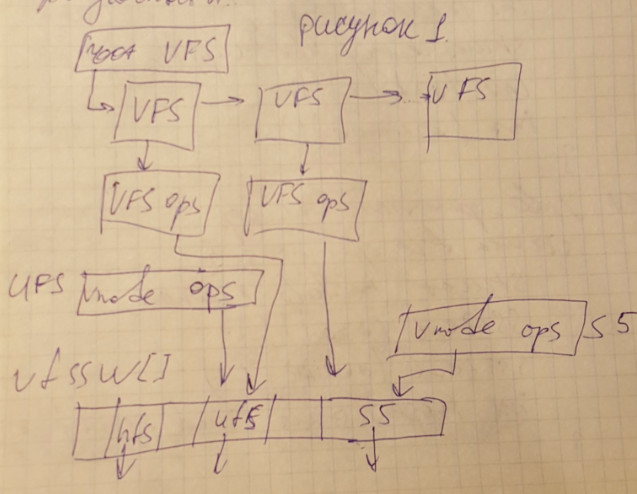
\includegraphics[width=\textwidth]{pic/1.png}
  \caption{pic}
\end{figure}

\lstinputlisting[language=c, caption=listing]{listing/2.c} 

Суперблок – начальная точка любой ФС, содержит инфу о ФС. Хранится в специальном секторе диска и имеет структуру \verb|super_block|.

\lstinputlisting[language=c, caption=Структура суперблок ]{listing/3.c} 

Структура суперблок одна из двух структур, в которой хранится инфа о смонтированных ФС. Вторая – \verb|struct vfs mount|. Это сделано, чтобы можно было смонтировать в разные ???. Доступ к суперблоку должен быть монопольным.

\lstinputlisting[language=c, caption=Операции на суперблоке]{listing/4.c} 

В "/fs/super.c" код для создания/управления/ликвидации объекта суперблок.

Объект суперблок создается и инициируется в ???loc.super() которая вызывается при монтировании ФС. Эта функция считывает суперблок ФС и запоминает поля созданного объекта. 
Битовая карта блоков – структура, каждый бит показывает, отведен ли соответствующий блок какому либо файлу. Если 1 – то блок занят.
ilist битовая карта индексных дескрипторов выполняет аналогичную функцию по отношению к ??? и показывает, какие индексные дескрипторы заняты. inode – кэшируется (хранится на диске и ядре, в ядре имеет таблицу актуальных inode).

Реализация inode cache для Linux находится в единственном файле $fs/inode.c$.
Inode cache в Linux представляет из себя:
\begin{enumerate}
	\item Глобальный хеш-массив \verb|inode_hashtable|, в котором каждый inode хешируется по значению указателя на суперблок и 32-битному номеру inode. При отсутствии суперблока (\verb|inode->i_sb == NULL|), вместо хеш-массива inode добавляется к двусвязному списку \verb|anon_hash_chain|. Примером таких анонимных inodes могут служить сокеты, созданные вызовом функции \verb|net/socket.c:sock_alloc()|, которая вызывает \verb|fs/inode.c:get_empty_inode()|.
	\item Глобальный список \verb|inode_in_use|, который содержит допустимые inodes (\verb|i_count > 0| и \verb|i_nlink > 0|). Inodes вновь созданные вызовом функций \verb|get_empty_inode()| и \verb|get_new_inode()| добавляются в список \verb|inode_in_use|
	\item Глобальный список \verb|inode_unused|, который содержит допустимые inode с \verb|i_count = 0|.
	\item Список для каждого суперблока (\verb|sb->s_dirty|) , который содержит inodes с \verb|i_count > 0|, \verb|i_nlink > 0| и \verb|i_state & I_DIRTY|. Когда inode помечается как "грязный" (здесь и далее под термином "грязный" подразумевается "измененный"), он добавляется к списку \verb|sb->s_dirty| при условии, что он (inode) хеширован. Поддержка такого списка позволяет уменьшить накладные расходы на синхронизацию.
	\item Inode cache суть есть - SLAB cache, который называется \verb|inode_cachep|. Объекты inode могут создаваться и освобождаться, вставляться и изыматься из SLAB cache
\end{enumerate}

Через поле \verb|inode->i_list| с inode вставляется в список определенного типа, через поле \verb|inode->i_hash| - в хеш-массив. Каждый inode может входить в хеш-массив и в один и только один список типа (\verb|in_use|, $unused$ или $dirty$).

Системный вызов $open$ реализован в виде функции \verb|fs/open.c:sys_open|, но основную работу выполняет функция \verb|fs/open.c:filp_open()|, которая разбита на две части:
\begin{enumerate}
	\item \verb|open_namei()|: заполняет структуру \verb|nameidata|, содержащую структуры \verb|dentry| и \verb|vfsmount|.
	\item \verb|dentry_open()| с учетом \verb|dentry| и \verb|vfsmount|, размещает новую структуру \verb|file| и связывает их между собой; вызывает метод \verb|f_op->open()| который был установлен в \verb|inode->i_fop| при чтении inode в \verb|open_namei()| (поставляет inode через \verb|dentry->d_inode|).
\end{enumerate}

Функция \verb|open_namei()| взаимодействует с dentry cache, в результате найдётся вход в родительский каталог и получится соответствующий inode вызовом \verb|iget(sb, ino)|.

Таким образом, при открытии файла вызывается \verb|iget(sb, ino)|, которая, фактически, называется \verb|iget4(sb, ino, NULL, NULL)|, эта функция:
\begin{enumerate}
	\item Пытается найти inode в хеш-таблице по номерам суперблока и inode. Поиск выполняется под блокировкой \verb|inode_lock|. Если inode найден, то увеличивается его счетчик ссылок (\verb|i_count|); если счетчик перед инкрементом был равен нулю и inode не "грязный", то он удаляется из любого списка (\verb|inode->i_list|), в котором он находится (это конечно же список \verb|inode_unused|) и вставляется в список \verb|inode_in_use|; в завершение, уменьшается счетчик \verb|inodes_stat.nr_unused|.
	\item дальше не успели, но можно посмотреть на \cite{rus-linux.net_VFS}
\end{enumerate}


